\section{Analysis}
		\subsection{Loss Function}
	From the reference \cite{ref3}, we can know that there exist various ways to evaluate the accuracy of a neural network. For simplicity, this program uses MSE (Mean-Square-Error) to be our loss function to evaluate the accuracy of the neural network. The equation is shown below:
	\begin{equation}
	    \textrm{MSE} = (\frac{1}{n})\sum_{i=1}^{n}\left(y_i - \hat{y_i}\right)^2  
	\end{equation}
	where $y_i$ is the actual training output and $\hat{y_i}$ is the desired output.   
	\subsection{Graph Display}
	The graph below shows the loss function with sample training iterations (30000 times). 
	\begin{figure}[h]
	    \centering
	    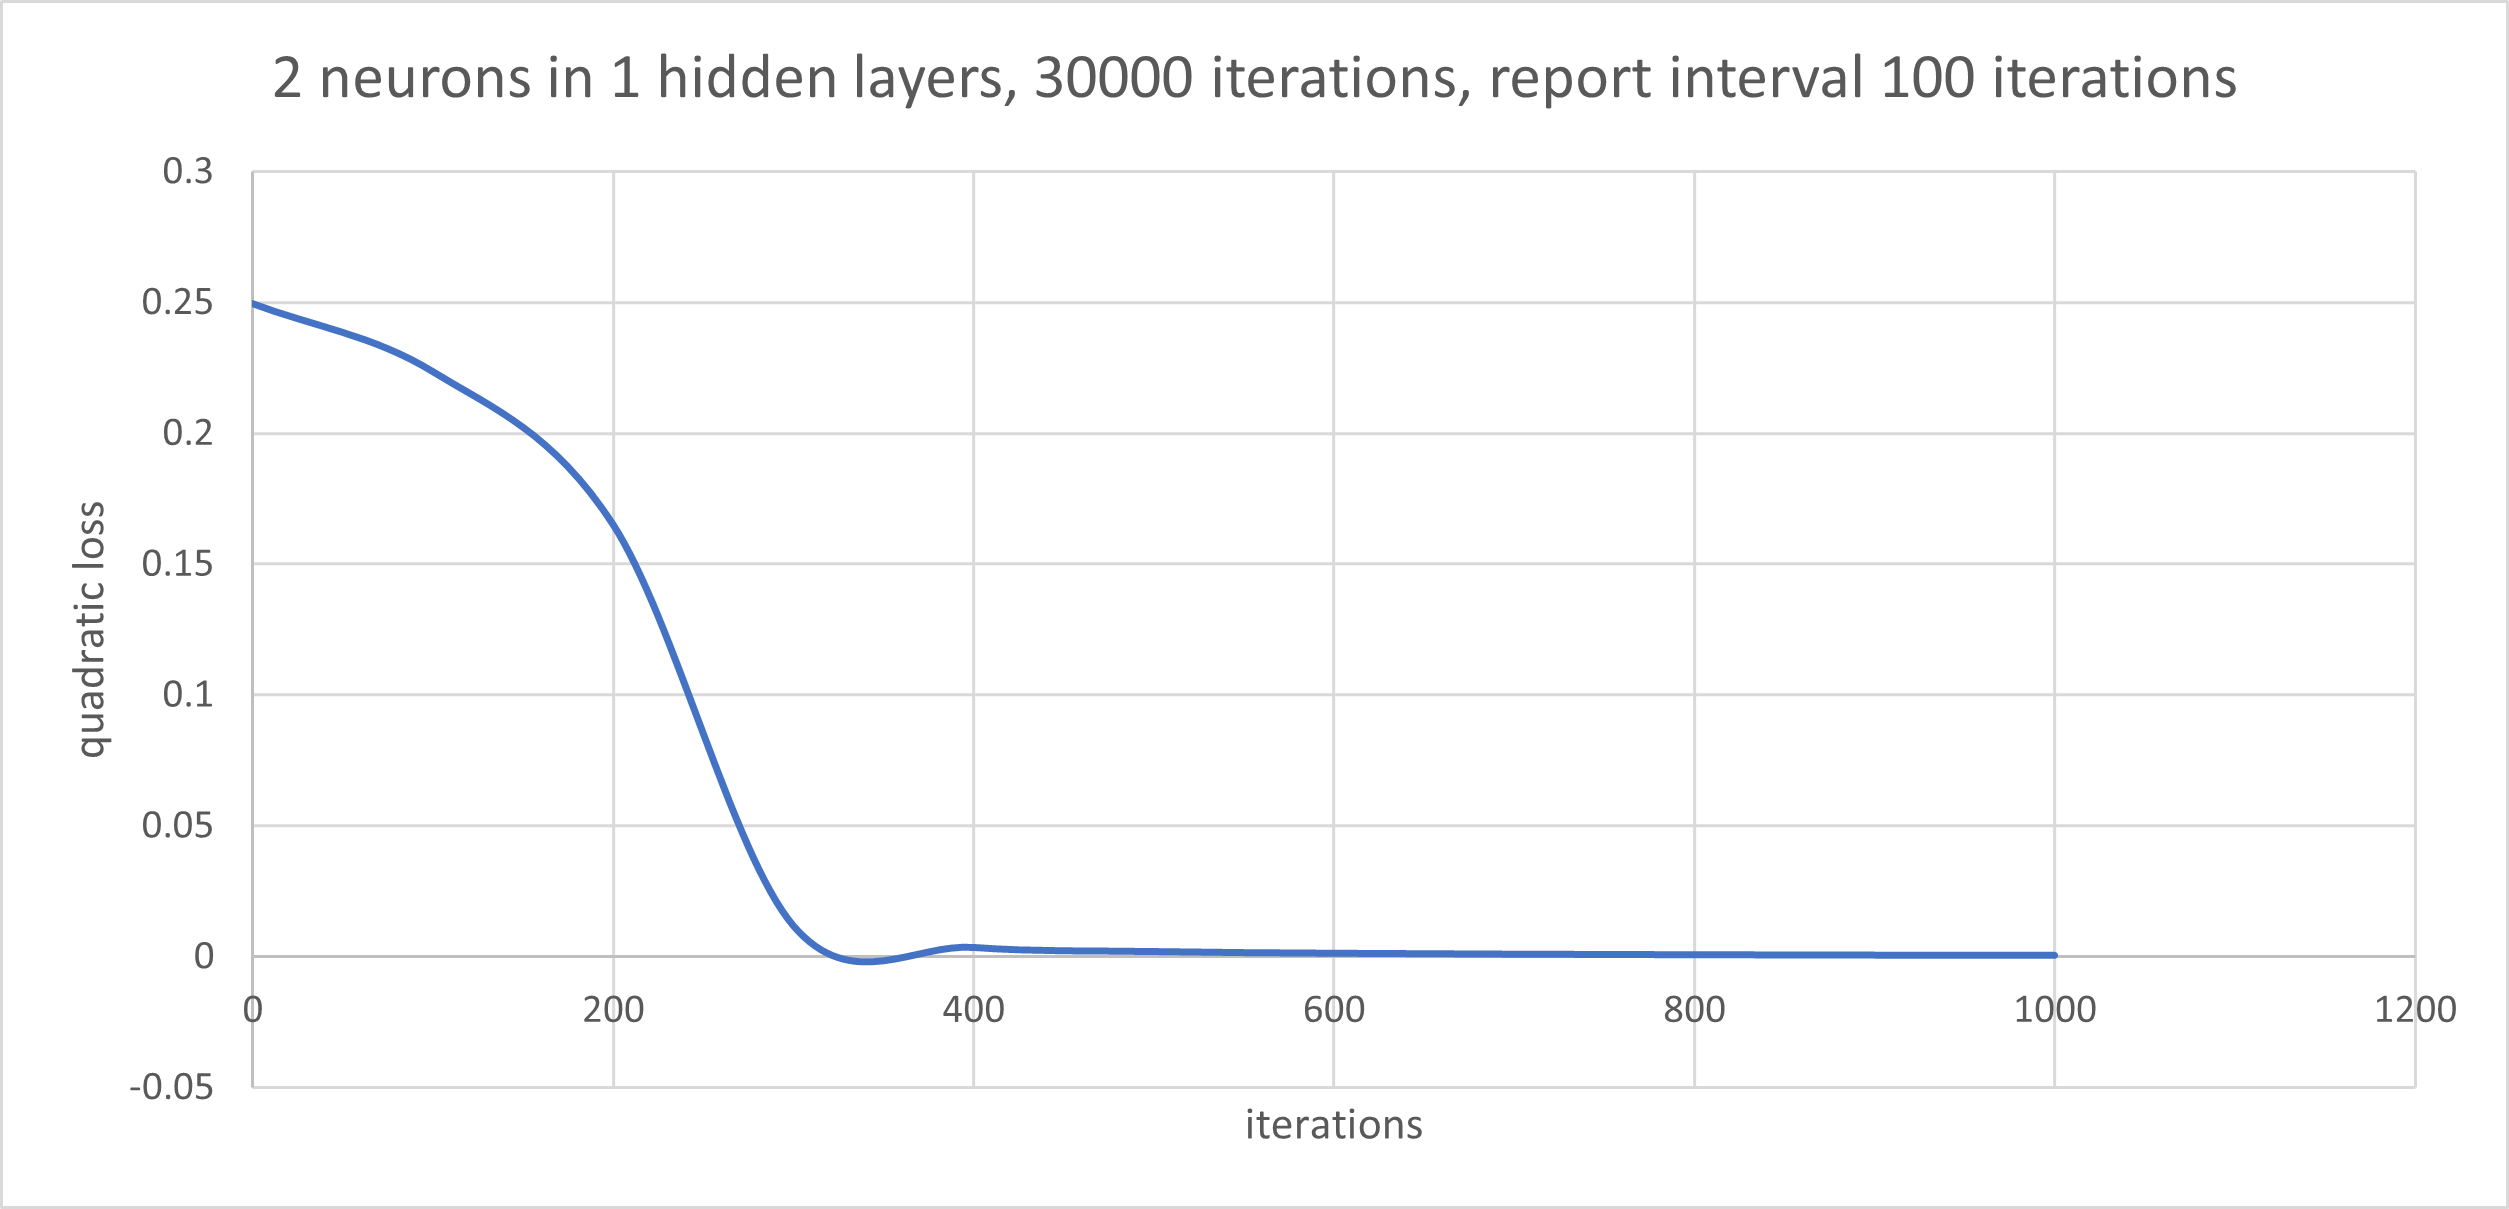
\includegraphics[width=1\textwidth]{image/2in1.png}
	    \caption{Graphs of Loss Function: MSE v.s. iterations}
	    \label{fig:my_label}
	\end{figure}
	\\Note that this graph only shows up to 1000 iterations since the value after 1000 iterations approaches zero and is trivial. The graph at first reached its highest value (approximately 0.25), and then gradually falls down to zero with the increase of training epochs. 
	\subsection{Further Improvement}
	Although the program has been successfully executed, there are still some issues to be fixed, listed below:
	\begin{itemize}
	    \item a CSV output of the loss function could be added when training completes.
	    \item Data storage of bits can be reduced to \lstinline{bool} array instead of \lstinline{char} array to reduce memory. 
	    \item In \lstinline{void getBitString()} : the string of bits can be the function's return value. Doing this may clarify the workflow of  \lstinline{void getRealAns()} and \lstinline{void getTrainAns()}. 
	\end{itemize}